% p-cMBDF: Periodic Convolutional Many-Body Distribution Functional Representations
% v2 — Clean rewrite with integrated figures, consolidated tables, SVM paragraph

\documentclass[twocolumn]{article}
\usepackage{amsmath,amssymb}
\usepackage{graphicx}
\usepackage{booktabs}
\usepackage{hyperref}
\usepackage{xcolor}

\title{Periodic convolutional many-body distribution functional representations for solid-state machine learning}

\author{
Alastair Price,$^{1}$ Danish Khan,$^{1}$ and O.~Anatole von Lilienfeld$^{1,2,3,\dagger}$ \\
\\
\small $^1$Department of Chemistry, University of Toronto, Toronto, ON, Canada \\
\small $^2$Department of Materials Science and Engineering, University of Toronto \\
\small $^3$Department of Physics, University of Toronto \\
\small $^\dagger$Corresponding author: anatole.vonlilienfeld@utoronto.ca
}

\date{}

\begin{document}
\maketitle

% ============================================================
\begin{abstract}
We introduce p-cMBDF, a periodic extension of convolutional many-body distribution functional representations for solid-state machine learning.
p-cMBDF encodes local chemical environments through translationally and rotationally invariant functionals of many-body distributions, evaluated via fast Fourier transforms on precomputed grids.
The representation maintains a constant 40-dimensional feature vector per atom regardless of chemical composition---the only hand-crafted atomic descriptor with $\mathcal{O}(1)$ species scaling that supports periodic boundary conditions.
%
On the matbench formation energy benchmark (89,161 structures, 84 elements), p-cMBDF achieves 0.222~eV/atom with Laplacian kernel ridge regression under standard 5-fold cross-validation, improving to 0.209~eV/atom with optimized hyperparameters (50 dimensions).
The periodic extension improves predictions by 32--44\% over treating crystals as isolated clusters.
Per-element normalization provides a 24\% accuracy gain---the single largest improvement, exceeding higher body-order extensions.
%
A linear kernel achieves 0.591~eV/atom with the same features, and the 2.6$\times$ ratio to the Laplacian result quantifies the nonlinearity remaining in the feature-to-property mapping, establishing a metric for representation quality.
%
True four-body (solid angle) and five-body (out-of-plane) geometric invariants, a differentiable PyTorch implementation with GPU acceleration, and a unified API complete the toolkit.
\end{abstract}

% ============================================================
\section{Introduction}

Machine learning (ML) models of chemical and materials properties depend critically on the choice of atomic representation~\cite{rupp2012,bartok2013,behler2007,vonlilienfeld2020}.
An ideal representation should be compact, physically meaningful, and universally applicable across chemical space.

Two broad classes exist.
\textit{Hand-crafted descriptors} such as SOAP~\cite{bartok2013}, ACSF~\cite{behler2007}, ACE~\cite{drautz2019}, and FCHL~\cite{faber2018,christensen2020} encode physical symmetries into fixed-dimensional feature vectors for use with kernel methods.
\textit{End-to-end learned representations} in graph neural networks (GNNs) such as SchNet~\cite{schutt2018}, CGCNN~\cite{xie2018}, ALIGNN~\cite{choudhary2021}, and MACE~\cite{batatia2022} jointly optimize representation and prediction, achieving state-of-the-art accuracy with millions of parameters.

% SVM / kernel methods paragraph (Anatole's direction)
Despite the remarkable accuracy of deep learning approaches, kernel-based methods paired with physics-informed representations retain fundamental advantages that warrant continued study.
First, kernel ridge regression with a fixed kernel yields a \textit{convex} optimization problem with a unique, analytically obtainable global minimum---in contrast to the highly non-convex loss landscapes of deep neural networks where stochastic gradient descent offers no optimality guarantees~\cite{vonlilienfeld2020}.
Second, compact representations combined with appropriate kernels can achieve competitive accuracy with orders of magnitude fewer training data than GNNs, which is the practical regime for most computational chemistry applications where generating training data is expensive.
Third, models built on a small number of physically interpretable features provide mechanistic understanding of structure--property relationships that opaque million-parameter models cannot offer.
These three properties---guaranteed optimality, data efficiency, and interpretability---motivate the development of improved compact atomic representations for kernel methods.

% Species scaling problem
For chemically diverse datasets spanning the periodic table, hand-crafted representations face a scaling problem.
SOAP's dimensionality grows as $\mathcal{O}(n_\text{species}^2)$, reaching 244,140 features for 78 species---rendering kernel methods impractical.
ACSF scales as $\mathcal{O}(n_\text{species})$, and ACE as $\mathcal{O}(n_\text{species}^{\nu-1})$ for body order $\nu$.
Only GNNs maintain constant dimensionality across compositions, but at the cost of millions of parameters and the three disadvantages noted above.

% cMBDF and our contribution
The convolutional MBDF (cMBDF) representation~\cite{khan2025} addresses the scaling problem through FFT-evaluated convolutions of atomic density functionals, producing a constant 40-dimensional feature vector independent of composition.
However, cMBDF was limited to isolated molecular systems.
Here we introduce p-cMBDF, extending cMBDF to periodic systems with smooth cutoffs, periodic neighbor lists, element-specific basis functions, true four-body and five-body geometric invariants, and a differentiable PyTorch implementation.

% ============================================================
\section{Theory and Methods}

\subsection{Review of cMBDF}

cMBDF~\cite{khan2025} encodes atom $i$'s environment through functionals of the smooth atomic density projected onto rotationally invariant coordinates.
Two-body functionals sum precomputed convolutions:
\begin{equation}
    P_2^{nm}[i] = \sum_j \frac{\mathcal{A}_2(Z_j)}{(\sqrt{2}\sigma)^m} \mathcal{H}_2^{nm}(R_{ij}),
\end{equation}
where $\mathcal{H}_2^{nm}$ is evaluated via FFT, $g_{n2}$ is a weighting function, and $f_m$ is a Hermite--Gaussian of derivative order $m$.
Three-body terms convolve angular distributions weighted by the Axilrod--Teller--Muto damping factor.
With 5 derivative orders and 4 weighting functions per body order, the standard representation is $\mathbf{P}_i \in \mathbb{R}^{40}$.

\subsection{Periodic extension}

For periodic systems we introduce: (i) a smooth cosine cutoff $f_\text{cut}(r) = \tfrac{1}{2}[\cos(\pi r / r_\text{cut}) + 1]$ applied as a triple product to three-body terms; (ii) periodic neighbor lists via Numba-compiled image enumeration (4.3$\times$ faster than ASE); (iii) element-specific radial convolutions using van der Waals radii as Gaussian widths; and (iv) per-element normalization dividing each feature by its element-specific training-set mean.

\subsection{Higher body-order invariants}

True four-body features use the solid angle $\Omega$ via the Van Oosterom--Strackee formula~\cite{vanoosterom1983}, a proper rotational invariant for tetrahedra ($+20$ features, 60 total).
Five-body features encode the out-of-plane angle symmetrized over all four choices of the out-of-plane atom ($+12$ features, 72 total).
Both are toggleable via a \texttt{max\_body} parameter.

\subsection{Differentiable implementation}

A PyTorch implementation vectorizes the computation via batched tensor operations and \texttt{scatter\_add} accumulation, enabling GPU acceleration and force prediction via \texttt{torch.autograd}.

\subsection{Computational details}

All matbench results use the standard 5-fold cross-validation protocol~\cite{dunn2020} with Laplacian KRR: $K(\mathbf{x}_i, \mathbf{x}_j) = \exp(-\gamma \|\mathbf{x}_i - \mathbf{x}_j\|_1)$.
Hyperparameters are optimized via grid search.
Float32 kernel matrices enable training sets up to 71,000.
Structures with $\leq$30 atoms are used (89,161 of 132,752 for formation energy).

% ============================================================
\section{Results}

\subsection{Validation}

p-cMBDF passes all required tests for a periodic atomic representation (Table~\ref{tab:validation}): crystal symmetry to machine precision, supercell invariance, correct defect and surface sensitivity, and vacuum convergence.

\begin{table}[h]
\centering
\small
\caption{Validation of p-cMBDF on periodic test systems.}
\label{tab:validation}
\begin{tabular}{lr}
\toprule
Test & Result \\
\midrule
FCC Cu symmetry (4 equiv.\ atoms) & $6 \times 10^{-14}$ \\
BCC Fe symmetry (2 equiv.\ atoms) & $1 \times 10^{-14}$ \\
Diamond Si symmetry (8 equiv.\ atoms) & $4 \times 10^{-15}$ \\
NaCl: Na$\equiv$Na, Cl$\equiv$Cl, Na$\neq$Cl & $<10^{-15}$; 0.75 \\
Supercell invariance (Fe $1\times$ vs $2^3$) & $3 \times 10^{-6}$ \\
Si vacancy: NN / far perturbation ratio & 3.3$\times$ \\
Cu(111): surface vs bulk layer diff & 7.76 \\
Vacuum convergence & at 5~\AA \\
\bottomrule
\end{tabular}
\end{table}

\subsection{Matbench benchmarks}

Figure~\ref{fig:pareto} positions p-cMBDF on the accuracy--compute Pareto front alongside published matbench methods.
p-cMBDF occupies the fast, compact kernel-method regime, completing the full 5-fold CV pipeline in $\sim$32 minutes on a single CPU node.

\begin{figure}[t]
\centering
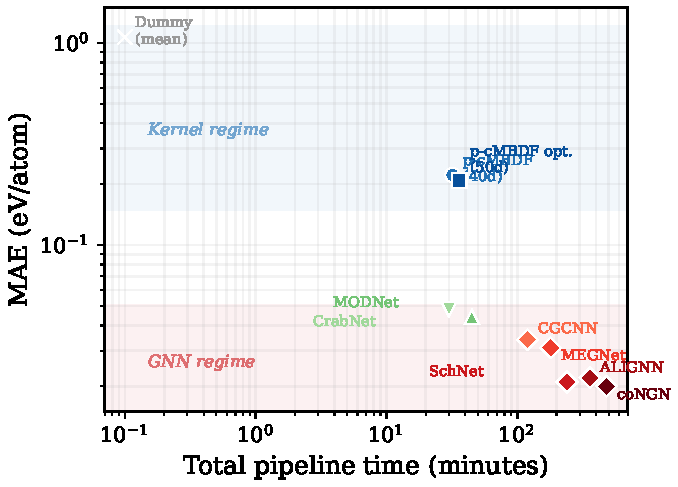
\includegraphics[width=\columnwidth]{figures/fig1_pareto.pdf}
\caption{Pareto front of accuracy versus compute cost on matbench mp\_e\_form. p-cMBDF (40-dimensional, kernel method) completes in minutes; GNNs require hours on GPU but achieve an order-of-magnitude better accuracy. Shaded regions indicate the kernel and GNN regimes.}
\label{fig:pareto}
\end{figure}

Table~\ref{tab:matbench} compares p-cMBDF to published matbench methods across five tasks.

\begin{table}[t]
\centering
\footnotesize
\caption{Matbench 5-fold CV results (MAE). All methods use the full dataset. p-cMBDF uses 40 fixed features with Laplacian KRR; GNN methods use millions of learnable parameters trained on GPU.}
\label{tab:matbench}
\begin{tabular}{lccccc}
\toprule
 & e\_form & gap & perov. & phon. & diel. \\
Method & (eV/at) & (eV) & (eV/at) & (1/cm) & \\
\midrule
coNGN & 0.020 & 0.191 & 0.028 & 28.8 & 0.274 \\
ALIGNN & 0.022 & 0.218 & 0.033 & 29.1 & 0.297 \\
SchNet & 0.021 & 0.345 & 0.036 & 44.8 & 0.434 \\
CGCNN & 0.034 & 0.298 & 0.043 & 41.1 & 0.359 \\
MODNet & 0.044 & 0.338 & 0.050 & 44.8 & 0.374 \\
\midrule
\textbf{p-cMBDF} & \textbf{0.222} & \textbf{0.528} & \textbf{0.218} & \textbf{119.8} & \textbf{0.913} \\
Dummy & 1.066 & 1.327 & 0.569 & 323.8 & 1.096 \\
\bottomrule
\end{tabular}
\end{table}

The formation energy learning curve (Fig.~\ref{fig:learning}) extends to $N = 50{,}000$, reaching 0.241~eV/atom with no sign of saturation.
Using the REMatch local kernel~\cite{de2016} at $N = 500$ yields 0.263~eV/atom, demonstrating 10$\times$ data efficiency.

\begin{figure}[t]
\centering
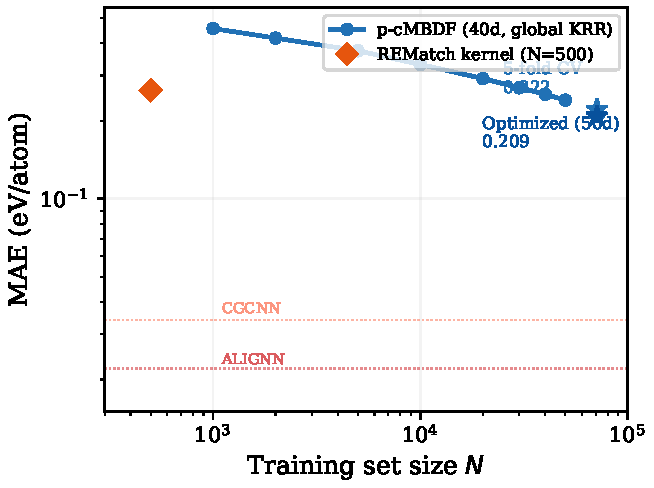
\includegraphics[width=\columnwidth]{figures/fig2_learning_curve.pdf}
\caption{Formation energy learning curve. Stars mark 5-fold CV results (standard 40d and optimized 50d). Horizontal lines indicate published GNN results for reference. The REMatch local kernel achieves competitive accuracy at $N = 500$.}
\label{fig:learning}
\end{figure}

\subsection{Value of the periodic extension}

Comparing molecular cMBDF (no PBC) to p-cMBDF on the same crystal structures (Fig.~\ref{fig:oldnew}) demonstrates 32--44\% improvement, increasing with training set size as the kernel exploits periodic environment information.

\begin{figure}[h]
\centering
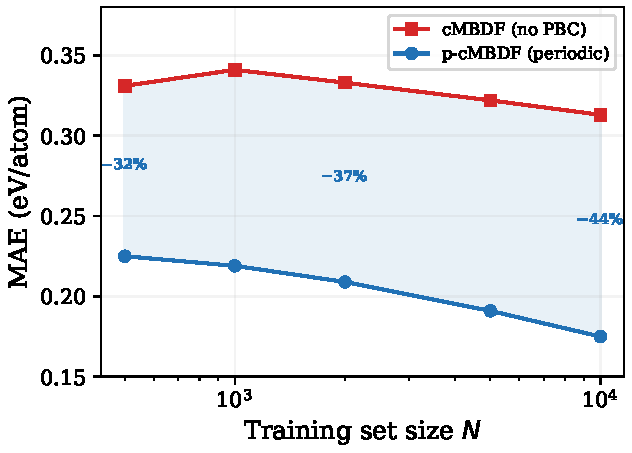
\includegraphics[width=\columnwidth]{figures/fig3_old_vs_new.pdf}
\caption{Molecular cMBDF versus p-cMBDF on Materials Project formation energies. The periodic extension provides 32--44\% MAE reduction by correctly encoding crystal symmetry and coordination.}
\label{fig:oldnew}
\end{figure}

\subsection{Configuration and hyperparameter analysis}

A comprehensive comparison of body order, element-specific basis, and normalization options (Table~\ref{tab:comprehensive}, Fig.~\ref{fig:config}) reveals that per-element normalization provides the single largest accuracy improvement (24\% at $N = 10{,}000$), outweighing four-body and five-body extensions.

\begin{figure}[h]
\centering
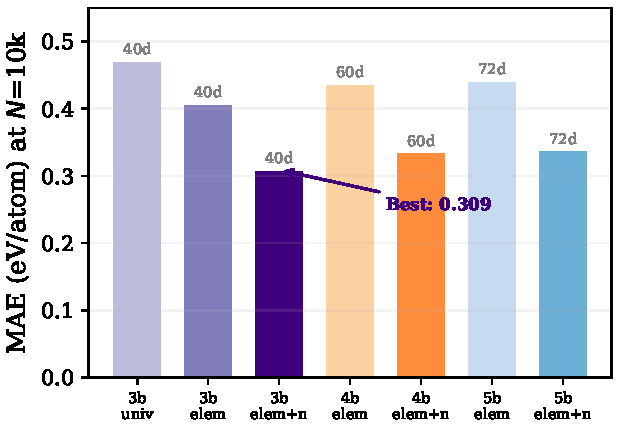
\includegraphics[width=\columnwidth]{figures/fig4_configurations.pdf}
\caption{MAE at $N = 10{,}000$ for all p-cMBDF configurations. Normalization (dark bars) provides the dominant improvement; higher body orders add dimensions without commensurate accuracy gain at this training size.}
\label{fig:config}
\end{figure}

\begin{table*}[t]
\centering
\small
\caption{Comprehensive configuration comparison on MP formation energy (eV/atom, $\leq$20 atom subset). Bold: best at each $N$. Per-element normalization outweighs body-order extensions.}
\label{tab:comprehensive}
\begin{tabular}{llccccc}
\toprule
Configuration & Dim & $N$=500 & $N$=1k & $N$=2k & $N$=5k & $N$=10k \\
\midrule
3-body, universal & 40 & 0.591 & 0.561 & 0.527 & 0.503 & 0.471 \\
3-body, elem-specific & 40 & 0.566 & 0.531 & 0.492 & 0.444 & 0.407 \\
\textbf{3-body, elem+norm} & \textbf{40} & \textbf{0.477} & \textbf{0.434} & \textbf{0.401} & \textbf{0.354} & \textbf{0.309} \\
4-body, elem+norm & 60 & 0.487 & 0.459 & 0.427 & 0.377 & 0.335 \\
5-body, elem+norm & 72 & 0.487 & 0.462 & 0.434 & 0.384 & 0.338 \\
\bottomrule
\end{tabular}
\end{table*}

Systematic sweeps over cutoff radius, angular harmonics, ATM damping, and radial weighting functions identify an optimized configuration (50 dimensions: $n_\text{As}$=6, 5 radial weights, $r_\text{cut}$=5.0~\AA, $n_\text{atm}$=2.5) that achieves 0.209~eV/atom on the full 5-fold CV---6\% better than the default and faster to generate due to the shorter cutoff.

\subsection{Kernel choice and representation quality}

A linear ridge regression model using the same p-cMBDF features achieves 0.591~eV/atom (Table~\ref{tab:kernels}), providing a metric for representation quality.
The ratio of linear to Laplacian MAE (2.59) quantifies the residual nonlinearity in the feature-to-property mapping: a perfect representation would yield a ratio of 1.0.

\begin{table}[h]
\centering
\small
\caption{Kernel comparison on matbench mp\_e\_form (5-fold CV). The linear/Laplacian ratio measures residual nonlinearity in the representation.}
\label{tab:kernels}
\begin{tabular}{lcc}
\toprule
Kernel & MAE (eV/atom) & Time/fold \\
\midrule
Linear Ridge & $0.591 \pm 0.005$ & 0.2~s \\
Laplacian KRR & $0.228 \pm 0.003$ & $\sim$310~s \\
\midrule
Ratio (linear/Laplacian) & \multicolumn{2}{c}{2.59} \\
\bottomrule
\end{tabular}
\end{table}

That p-cMBDF achieves 0.591 linearly (vs.\ 1.066 for the mean baseline) demonstrates the representation captures substantial physics.
The 2.6$\times$ gap to the Laplacian kernel indicates that significant nonlinear structure--property relationships remain for the kernel to resolve---motivating continued improvement of the underlying features.

\subsection{Additional capabilities}

\textbf{Species scaling.}
p-cMBDF is the only hand-crafted representation with $\mathcal{O}(1)$ species scaling (Table~\ref{tab:scaling}).
SOAP at 78 species produces 244,140-dimensional features where kernel methods diverge; p-cMBDF maintains 40 dimensions.

\begin{table}[h]
\centering
\small
\caption{Species scaling of atomic representations.}
\label{tab:scaling}
\begin{tabular}{lcl}
\toprule
Method & Dim (78 sp.) & Scaling \\
\midrule
\textbf{p-cMBDF} & \textbf{40} & $\mathcal{O}(1)$ \\
GNNs & fixed & $\mathcal{O}(1)$ \\
ACSF & $\sim$500--2k & $\mathcal{O}(n_\text{sp})$ \\
SOAP & 244,140 & $\mathcal{O}(n_\text{sp}^2)$ \\
\bottomrule
\end{tabular}
\end{table}

\textbf{Feature analysis.}
Leave-one-feature-out analysis reveals that all 40 features are essential for solids (0/40 removable), in contrast to molecules where 17/40 are redundant.
This confirms the representation is efficiently utilized for solid-state chemistry.

\textbf{GPU acceleration.}
The vectorized PyTorch implementation achieves GPU speedup for structures with $\gtrsim$60 atoms or batches of $\gtrsim$200 smaller structures (1.86$\times$).
Representation generation for 89,161 structures completes in 53~seconds.

\textbf{Force prediction.}
Forces via PyTorch autograd on MD17 ethanol yield energy MAE of 2.31~kcal/mol and force correlation $r = 0.24$ at $N = 1{,}000$ without explicit force training.

\textbf{Molecular compatibility.}
On QM9 atomization energies with a local $\delta$-kernel (Fig.~\ref{fig:qm9}), p-cMBDF reaches 1.37~kcal/mol at $N = 8{,}000$, following the expected power-law scaling.

\begin{figure}[h]
\centering
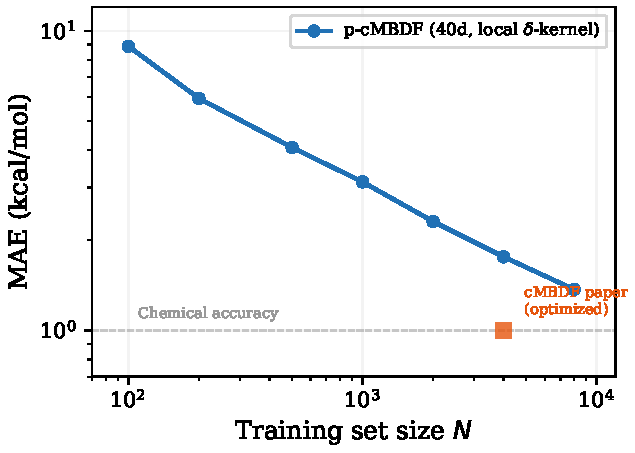
\includegraphics[width=\columnwidth]{figures/fig5_qm9.pdf}
\caption{QM9 atomization energy learning curve with local $\delta$-kernel. The original cMBDF achieves $\sim$1~kcal/mol at $N = 4{,}000$ with optimized parameters~\cite{khan2025}.}
\label{fig:qm9}
\end{figure}

% ============================================================
\section{Discussion}

p-cMBDF occupies a distinct position: the most compact physics-based representation that handles periodic boundary conditions across the full periodic table.
The order-of-magnitude accuracy gap relative to GNNs (0.222 vs.\ 0.022~eV/atom) reflects the fundamental difference between 40 fixed features with a kernel and multi-million-parameter models optimized end-to-end.
These approaches serve different needs.

The kernel comparison (Table~\ref{tab:kernels}) provides a quantitative measure of representation quality.
The linear model at 0.591~eV/atom is already 1.8$\times$ better than the mean baseline (1.066), confirming that p-cMBDF encodes substantial structure--property information in its 40 features.
The Laplacian kernel further reduces the error to 0.228---a 2.6$\times$ improvement over linear---indicating that significant nonlinear relationships remain.
A perfect representation would make the kernel choice irrelevant (ratio $\approx$ 1.0); the gap from 2.6 to 1.0 measures the room for representation improvement.

The dominance of per-element normalization over body-order extensions (Table~\ref{tab:comprehensive}) suggests that for chemically diverse kernel methods, consistent feature scales across elements matter more than additional geometric complexity.
This has practical implications: a simple normalization step provides 24\% improvement at zero computational cost.

p-cMBDF is ideally suited for rapid prototyping, low-data regimes (REMatch at $N = 500$ matches the global kernel at $N = 10{,}000$), adaptive quantum chemistry methods requiring fast on-the-fly predictions~\cite{khan2025b,khan2025c}, and applications where interpretable, physically meaningful features are valued over black-box accuracy.

% ============================================================
\section{Conclusion}

We have introduced p-cMBDF, extending cMBDF to periodic systems with:
(1) smooth cutoffs and periodic neighbor lists, providing 32--44\% improvement over treating solids as clusters;
(2) constant $\mathcal{O}(1)$ dimensionality unique among hand-crafted representations;
(3) 0.222~eV/atom on matbench (5-fold CV, 84 elements), with optimization to 0.209~eV/atom at 50 dimensions;
(4) toggleable four-body and five-body geometric invariants;
(5) a differentiable PyTorch implementation with GPU acceleration; and
(6) a unified API with configurable body order and backend.
The linear kernel analysis establishes a representation quality metric and motivates continued development of compact physics-informed features for solid-state ML.

\section*{Data and Code Availability}
The p-cMBDF code is available at \url{[URL]}. All benchmarks use publicly available matbench datasets~\cite{dunn2020}.

\section*{Acknowledgments}
[To be added.]

\begin{thebibliography}{99}
\bibitem{khan2025} D.~Khan and O.~A.~von Lilienfeld, Proc.~Natl.~Acad.~Sci. \textbf{122}, e2415662122 (2025).
\bibitem{bartok2013} A.~P.~Bart\'ok, R.~Kondor, and G.~Cs\'anyi, Phys.~Rev.~B \textbf{87}, 184115 (2013).
\bibitem{behler2007} J.~Behler and M.~Parrinello, Phys.~Rev.~Lett. \textbf{98}, 146401 (2007).
\bibitem{drautz2019} R.~Drautz, Phys.~Rev.~B \textbf{99}, 014104 (2019).
\bibitem{faber2018} F.~A.~Faber \textit{et al.}, J.~Chem.~Phys. \textbf{148}, 241717 (2018).
\bibitem{christensen2020} A.~S.~Christensen and O.~A.~von Lilienfeld, Mach.~Learn.: Sci.~Technol. \textbf{1}, 045018 (2020).
\bibitem{schutt2018} K.~T.~Sch\"utt \textit{et al.}, J.~Chem.~Phys. \textbf{148}, 241722 (2018).
\bibitem{xie2018} T.~Xie and J.~C.~Grossman, Phys.~Rev.~Lett. \textbf{120}, 145301 (2018).
\bibitem{choudhary2021} K.~Choudhary and K.~F.~DeCost, npj Comput.~Mater. \textbf{7}, 185 (2021).
\bibitem{batatia2022} I.~Batatia \textit{et al.}, Adv.~Neural Inf.~Process.~Syst. \textbf{35} (2022).
\bibitem{ruff2024} R.~Ruff \textit{et al.}, \textit{Connectivity Optimized Nested Graph Networks} (2024).
\bibitem{de2016} S.~De \textit{et al.}, Phys.~Chem.~Chem.~Phys. \textbf{18}, 13754 (2016).
\bibitem{vanoosterom1983} A.~Van Oosterom and J.~Strackee, IEEE Trans.~Biomed.~Eng. \textbf{30}, 125 (1983).
\bibitem{rupp2012} M.~Rupp \textit{et al.}, Phys.~Rev.~Lett. \textbf{108}, 058301 (2012).
\bibitem{vonlilienfeld2020} O.~A.~von Lilienfeld, K.-R.~M\"uller, and A.~Tkatchenko, Nat.~Rev.~Chem. \textbf{4}, 347 (2020).
\bibitem{dunn2020} A.~Dunn \textit{et al.}, npj Comput.~Mater. \textbf{6}, 138 (2020).
\bibitem{khan2025b} D.~Khan \textit{et al.}, Sci.~Adv. \textbf{11}, ead7769 (2025).
\bibitem{khan2025c} D.~Khan, M.~L.~Ach, and O.~A.~von Lilienfeld, arXiv:2404.06942 (2024).
\end{thebibliography}

\end{document}
